\problemname{Smoke Signals}

\begin{figure}[h] 
\begin{center}
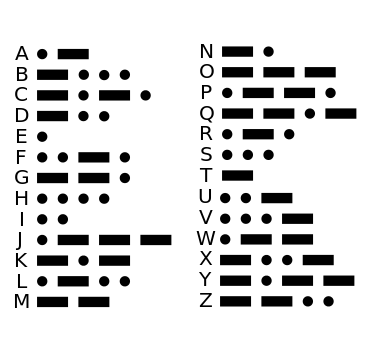
\includegraphics[width=8cm]{morse.png}
\caption{The Morse alphabet}
\end{center} 
\end{figure}

Your friend is out on a polar expedition, and to stay in touch she sends smoke signals encoded with Morse. You find it tiresome to learn the Morse alphabet by heart, and therefore want to write a program that translates the signal for you. The input is a string of ones and zeros, where a sequence of ones corresponds to a smoke cloud. Smoke clouds correspond to dashes and dots, and empty spaces correspond to pauses between dashes and dots, letters, and spaces.

\section*{Input}
The first $26$ lines contain a table of the Morse code for all letters.
Each such line contains a capital letter (A-Z), a space, and then the Morse encoding for that letter.

After the table follows a line with two distinct integers: $S$ and $P$.
$S$ is the number of ones that make up a dash, and $P$ is the number of ones that make up a dot.

Then comes a line with three distinct integers: $T$, $B$, and $M$.
$T$ zeros make up a pause between dot and dash, $B$ zeros signal a new letter, and $M$ zeros are a space.

Finally comes a line containing the number $N$, followed by an $N$-character long string of ones and zeros.

\section*{Output}
Your program shall output one line containing the decoded message.

\section*{Scoring}
Your solution will be tested on a set of test groups. To earn points for a group, you must pass all test cases in that group.
\begin{tabular}{| l | l | l | l |}
\hline
Group & Points & Constraints & Other \\ \hline
1     & 19         &  $S = 2, P = 1, T = 1, B = 2$, $1 \le N \le 200$  & No spaces occur\\ \hline
2     & 39         &  $1 \le S, P, T, B, M \le 10$, $1 \le N \le 2000$ & No spaces occur \\ \hline
3     & 25         &  $1 \le S, P, T, B, M \le 100$, $1 \le N \le 2000$    & \\ \hline
4     & 17        &  $1 \le S, P, T, B, M \le 1000$, $1 \le N \le 300\,000$  & \\ \hline
\end{tabular}
